\documentclass[a4paper]{article}
\usepackage[utf8]{inputenc}
\usepackage[spanish, es-tabla, es-noshorthands]{babel}
\usepackage[table,xcdraw]{xcolor}
\usepackage[a4paper, footnotesep = 1cm, width=20cm, top=2.5cm, height=25cm, textwidth=18cm, textheight=25cm]{geometry}
%\geometry{showframe}

\usepackage{tikz}
\usepackage{amsmath}
\usepackage{amsfonts}
\usepackage{amssymb}
\usepackage{float}
\usepackage{graphicx}
\usepackage{caption}
\usepackage{subcaption}
\usepackage{multicol}
\usepackage{multirow}
\setlength{\doublerulesep}{\arrayrulewidth}
\usepackage{booktabs}
\usepackage{mathrsfs,amsmath}
\usepackage{hyperref}
\hypersetup{
    colorlinks=true,
    linkcolor=blue,
    filecolor=magenta,      
    urlcolor=blue,
    citecolor=blue,    
}

\newcommand{\quotes}[1]{``#1''}
\usepackage{array}
\newcolumntype{C}[1]{>{\centering\let\newline\\\arraybackslash\hspace{0pt}}m{#1}}
\usepackage[american]{circuitikz}
\usetikzlibrary{calc}
\usepackage{fancyhdr}
\usepackage{units} 

\graphicspath{./Imagenes}

\pagestyle{fancy}
\fancyhf{}
\lhead{22.05 ASSD}
\rhead{Mechoulam, Lambertucci, Rodriguez, Londero}
\rfoot{Página \thepage}

\begin{document}

\subsection{Introducción modelo Karplus-Strong}
En esta sección se analizará el método de sintesis basado en el modelado físico, propuesto por Karplus-Strong.
\subsection{Karplus-Strong básico}
El modelo básico de Karplus-Strong consiste filtrar una forma de onda a travez de una linea de retardo, gracias a esto se logra simular el sonido de una cuerda de guitarra.
\begin{figure}[H]
	\centering
	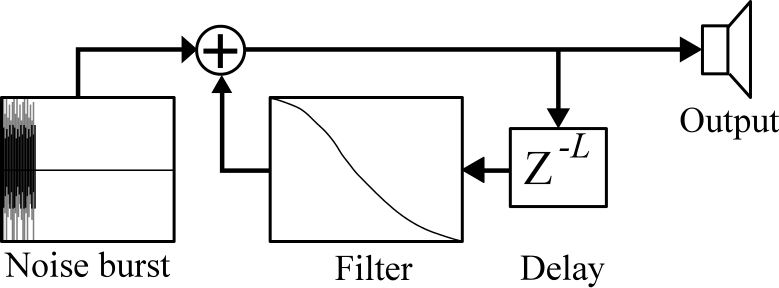
\includegraphics[width=0.8\textwidth]{ImagenesEjercicio4/ksinit.PNG}
\caption{Modelo clásico Karplus-Strong.}
	\label{fig:kscl}
\end{figure}
\subsubsection{Análisis teórico}
Este algoritmo se puede describir por su diagrama en bloques como se ve  a continuación.
\begin{figure}[H]
	\centering
	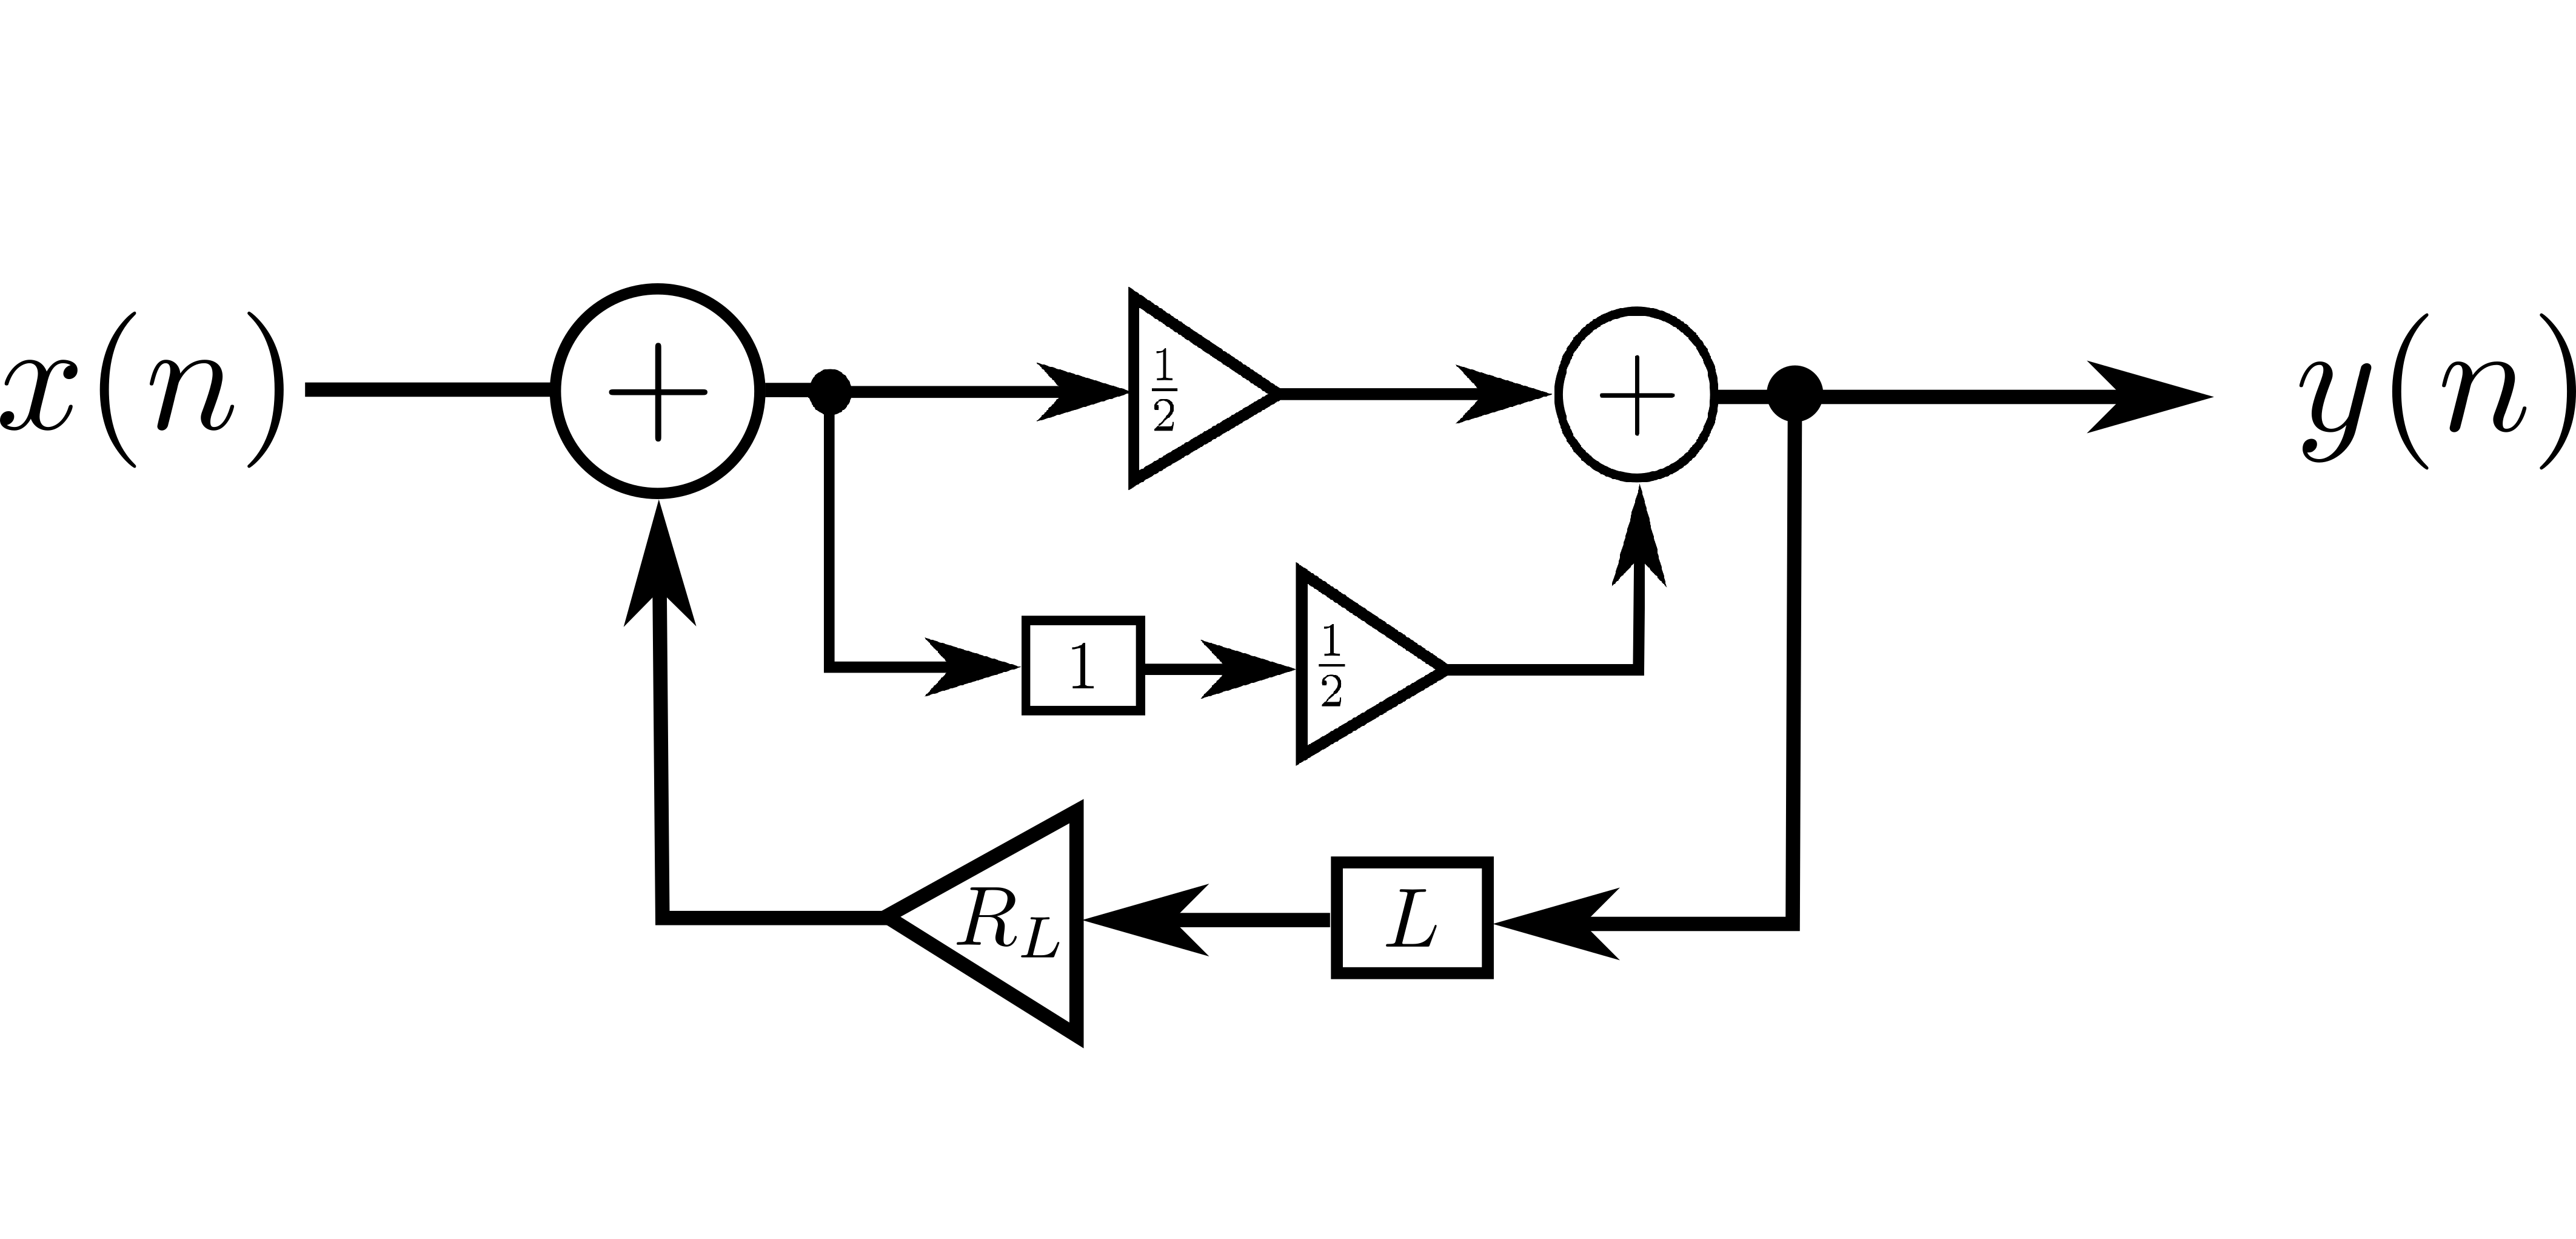
\includegraphics[width=0.8\textwidth]{ImagenesEjercicio4/ksclasic.PNG}
\caption{Algoritmo Karplus-Strong.}
	\label{fig:ksclasico}
\end{figure}
De este diagrama en bloques se puede obtener la ecuación en diferencias:
\begin{align}
y(n) = \frac{1}{2}\cdot x(n) +\frac{1}{2}\cdot x(n-1) + \frac{1}{2}\cdot R_L \cdot y(n-L) + + \frac{1}{2}\cdot R_L \cdot y(n-L-1) 
\label{eq:eqdif}
\end{align}
A partir de esta expresión se puede calcular su transformada Z y depejar para la transferencia:
\begin{align}
H(z) = \frac{\frac{1}{2} \cdot z^{L+1} +\frac{1}{2} \cdot z^{L} }{z^{L+1} - \frac{R_L}{2} \cdot z - \frac{R_L}{2}}
\label{eq:hzks}
\end{align}  
Vale la pena mencionar que de la ecuación (\ref{eq:eqdif}) es una ecuación en diferencias que cuenta como condiciones iniciales la wavetable suministrada por el ruido.
\subsubsection{Análisis singularidades}
Se observa que la expresión (\ref{eq:hzks}) cuenta con L+1 polos y L+1 ceros. A continuación se muestra un diagrama de polos y ceros del sistema:

\subsubsection{Sintonización de frecuencia}
\subsubsection{Tipos de ruido}
\subsubsection{Estabilidad}
La estabilidad del sistema será determinada por la ecuación (\ref{eq:hzks}) se puede observar que si RL es mayor o igual a uno el sistema será inestable, si bien teóricamente esto es cierto, en la realidad se encuentra que si RL = 1 no solo no provocará inestablidad, sino que es recomendable este valor dado que logrará extender las oscilaciones  un mayor tiempo.
\subsubsection{Cálculo Fase}
\subsection{Mejora propuesta}
\subsubsection{Análisis teórico}
\subsubsection{Sintonización de frecuencia}
\subsubsection{Continuidad del sonido}
\subsection{Karplus-Strong percución}
\subsection{Espectrogramas}
\end{document}